\begin{question}[section=2,name={18.1.2017},mode=exm,type=bsp,tags={20170118}]
	Eine kompensierte \textbf{Reihenschluss-Gleichstrommaschine} hat folgende Daten. Eine Leerlaufkennlinie $U_i/I_E$ bei $n=500 U/min$ ist gegeben.\\
	\begin{tabular}{L{2cm}l}
		$I_{A,N}$ \dotfill &$160~A$\\
		$U_{N}$ \dotfill & $200~V$ \\
		$n_N$ \dotfill & $1000~\frac{U}{min}$\\
	\end{tabular}
	\begin{enumerate}
		\item Wie groß ist die Spannungskonstante $k_1 \cdot \phi_N$ im Nennpunkt, das Nennmoment $M_N$ und die Nennleistung $P_N$ der Gleichstrommaschine? (\addpoints{2})
		\item Berechnen Sie den Innenwiderstand $R_i$ (=Ankerwiderstand $R_A$ + Erregerwiderstand $R_E$ ) und den Wirkungsgrad $\eta_N$ im Nennpunkt. (\addpoints{2})
		\item Bestimmen Sie die Drehzahl $n$ und das Drehmoment $M$ der Maschine für eine Ankerspannung $U_A =150~V$ und $I_A = 160~A$ (\addpoints{1})
		\item Skizzieren Sie die Drehzahl-Drehmoment Kennlinie ($M/n$) bei Nennspannung $U_{A,N}=200~V$ im Bereich ca. $0,2M_N$ bis $M_N$. (\addpoints{2})
		\item Die Maschine wird bei $n=500~U/min$ auf einen Widerstand $R_L$ gebremst. Dimensionieren Sie den Bremswiderstand $R_L$ so, dass ein anfänglicher Bremsstrom von $200~A$ ließt und geben Sie die Ankerspannung $U_A$ an den Maschinenklemmen und das Bremsmoment zu Beginn der Bremsung an. (\addpoints{3})
	\end{enumerate}
	\begin{figure}[H]
		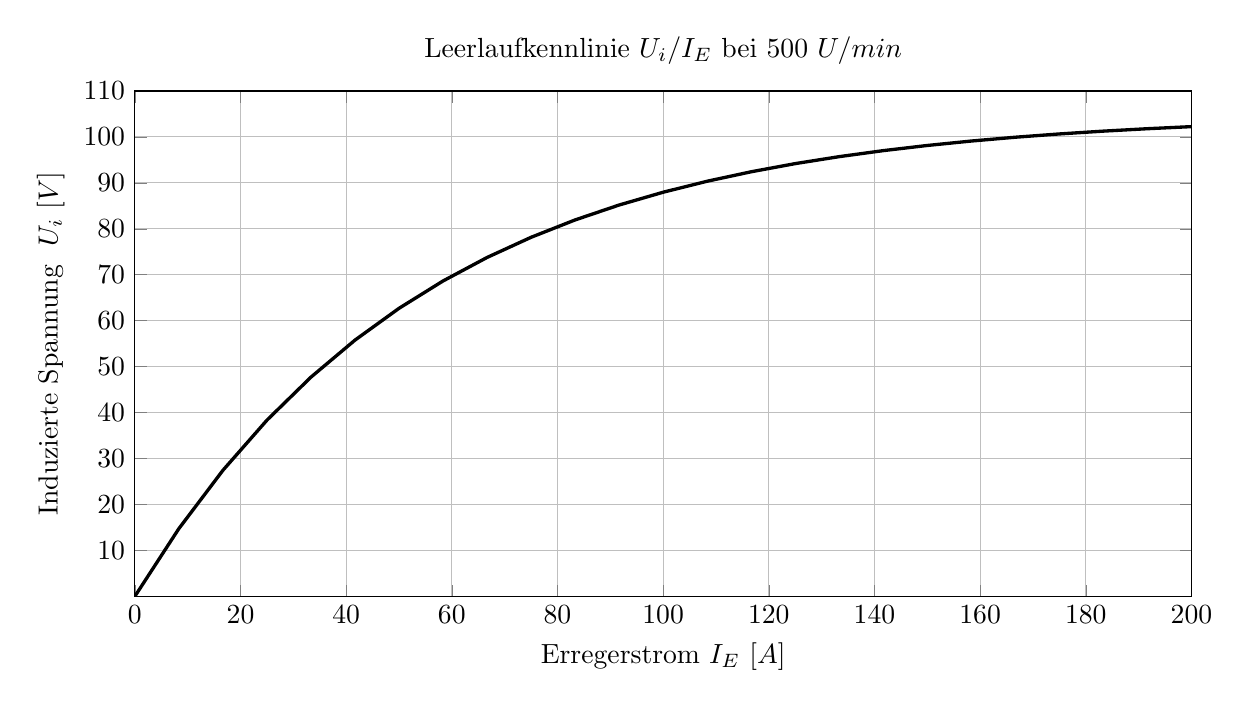
\begin{tikzpicture}
			\begin{axis}[title={{Leerlaufkennlinie} $U_i/I_E$ {bei} $500 ~U/min$},xlabel={{Erregerstrom }$I_E \, \left[A\right]$ }, ylabel={{Induzierte Spannung } $U_i \, \left [V\right]$},
				xtick= {0,20,40,60,80,100,120,140,160,180,200},width=15cm,height=8cm,
				xmin = 0,xmax = 200,
				ytick= {10,20,30,40,50,60,70,80,90,100,110},
				ymin = 0 , ymax = 110,grid=major]
				\addplot+
				[id=exp,color=black,mark=none,domain=0:200, very thick]{105*(1-exp(-x/55))};
				
			\end{axis}
		\end{tikzpicture}
		\caption{Leerlaufkennlinie} \label{fig:20170118}
	\end{figure}
\end{question}
\begin{solution}
	
\end{solution}